\documentclass[twoside,9pt,twocolumn]{aiaa}
% can use letter, twoside, oneside, 9pt, 10pt, 11pt, 12pt, onecolumn, twocolumn, conference, submit, mtpro
% aiaa conference papers should use the options oneside,10pt,letter,onecolumn,conference
\usepackage{graphicx}
\usepackage{rotating}
\usepackage{bm}


\newcommand{\alb}{\vspace{0.1cm}\\} % array line break
\newcommand{\mfd}{\displaystyle}
\renewcommand{\vec}[1]{\bm{#1}}

\author{  Daesu Oh\thanks{Graduate Student, Dept.\ of Aerospace Engineering, ohdaesu@pnu.edu} 
          ~and~ 
          B.\ Parent\thanks{Assistant Professor, Dept.\ of Aerospace Engineering, parent@pnu.edu}\\
          {\it Pusan National University, Busan 609-735, South Korea}\\
          ~and\\
          Mikhail Shneider\thanks{Research Staff Member, Dept.\ of Mechanical and Aerospace
                                  Engineering} 
          ~and 
          Sergey Macheret\thanks{Senior Research Scientist, Dept.\ of Mechanical and Aerospace
                                 Engineering, now at Lockheed Martin.}\\
          {\it Princeton University, Princeton, NJ 08544-5263, USA}\\}

\title{Example of a \LaTeX\ Article in AIAA Format}

\abstract{A new formulation of the generalized Ohm's law is here presented that is applicable to weakly-ionized plasmas with multiple types of ions. The novel formulation takes into consideration the separate ion slip currents associated with each type of ion and is recommended for computational studies of non-neutral and quasi-neutral weakly-ionized plasmas. Starting from the new form of the generalized Ohm's law, we derive an electric field potential equation that is applicable to a plasma with more than one type of ions. Despite some similarities between the potential equation and the Poisson equation, it is argued that the discretization of the potential equation cannot be accomplished in the same manner by using only central differences. It is here proven (and subsequently verified through a testcase) that when the plasma exhibits conjunctly a high Hall parameter and a high electrical conductivity gradient, the centered stencils introduce spurious oscillations which can lead to severe numerical error. Another contribution of this paper is to present a novel discretization of the potential equation which consists of a blend of central and upwind differences. The proposed scheme is consistently monotonic for any value of the Hall parameter and is second-order accurate except in the vicinity of discontinuities.  
}

\acknowledgments{Numerous discussions with Park Chan-Wook helped improve the quality of this manuscript considerably. This work was sponsored by a Pusan National University Grant.}
% use =acknowledgment{} for a single acknowledgment


\setlength\nomenclaturelabelwidth{0.43 in}

\nomenclature{

  \begin{nomenclaturelist}{Roman Symbols}
   \item[$a_i^{\rm SS}$]     wave speed associated with the skew-symmetric terms of the tensor conductivity
   \item[$\vec{B}$]          magnetic field vector
   \item[$\bar{\vec{B}}$]      normalized magnetic field vector, $\vec{B}/|\vec{B}|$
   \item[$C_k$]       charge of $k$th species
   \item[$\vec{E}$]          electric field vector
   \item[$N_k$]       number density of $k$th species
   \item[$s_k$]       sign of the charge, $-1$ for electrons and negative ions and $+1$ for positive ions
   \item[$\vec{v}$]          velocity vector of the bulk of the gas
   \item[$X_i$]       grid index along $x_i$ coordinate 
   \item[$x_i$]       spatial coordinate
   \item[$Y_k$]       matrix needed to determine the conductivity
  \end{nomenclaturelist}

  \begin{nomenclaturelist}{Greek Symbols}
   \item[$\sigma$]       scalar conductivity, $\sum |C_k| N_k \mu_k$
   \item[$\wtilde{\sigma}$]       tensorial conductivity
   \item[$\wtilde{\sigma}^{\rm S}$]       symmetric part of tensorial conductivity
   \item[$\wtilde{\sigma}^{\rm SS}$]       skew-symmetric part of tensorial conductivity
   \item[$\phi$]       electric field potential
   \item[$\beta_{\rm e}$]       Hall parameter for the electrons, $\mu_{\rm e} |\vec{B}|$
   \item[$\delta_{x_i}$]       discretization operator along  $x_i$ coordinate
   \item[$\Delta {x_i}$]       grid spacing along  $x_i$ coordinate
   \item[$\mu_k$]       mobility of $k$th species
  \end{nomenclaturelist}

}


\begin{document}
\maketitle
\makenomenclature

\section{Introduction}

\dropword Several applications of weakly-ionized plasma technologies for improving the performance of aircraft have recently been the subject of considerable interest.
One possible application is aerodynamic flow control through virtual bodies created by heat deposition using electron beams or another type of external ionizer \cite{jpp:2008:gaitonde,jpp:2008:shneider,jpp:2008:knight}.  Other applications are centered on the force exerted on the airflow due to magnetohydrodynamic interaction (MHD) or electrohydrodynamic interaction (EHD). The EHD interaction (or \emph{ion wind}) is suspected to be one of the mechanisms responsible for the high success of plasma actuators in preventing or delaying boundary layer separation \cite{aiaa:2009:roupassov}, in enhancing jet mixing \cite{aiaa:2008:benard}, in keeping the flow attached on turbine blades \cite{aiaa:2007:rizzetta}, or in controlling the vortices above a delta wing \cite{aiaa:2008:greenblatt}. On the other hand, the MHD interaction could be useful in controlling the inlet flowfield  \cite{aiaa:2002:shang,aiaaconf:2002:shneider}, in imparting momentum to a gas \cite{jpp:2005:parent,jpp:2007:parent}, or in generating electrical power aboard an aircraft through a MHD generator \cite{jpp:2009:fujino,aiaa:2009:wan}.
 
\subsection{EHD Interaction}
Despite some success using the weakly-ionized plasma technologies, there remain several key physical phenomena that are still not well understood. For instance, it is not clear whether plasma actuators achieve flow control through the EHD interaction or through heating, or how much of the Joule heating losses observed in a MHD generator occur within the plasma sheath. To obtain a better understanding of the physical phenomena, it is desirable to obtain more detailed computational results. 
%
\begin{table}[ht]
\fontsizetable
\begin{center}
  \begin{threeparttable}
    \tablecaption{$\epsilon$ and $\sigma$ for some species \tnote{1}}
    \fontsizetable
    \begin{tabular}{lllll}
      \toprule
species$_k$     &  ${\rm He}$    &  ${\rm H}_2$   &  ${\rm O}_2$   &  ${\rm N}_2$  \\
\midrule
$\epsilon_k$ [K]&  $10.22$       &  $59.7$        &  $106.7$       &  $71.4$       \\
$\sigma_k$ [nm] &  $0.2576$      &  $0.2827$      &  $0.3467$      &  $0.3798$     \\
      \bottomrule
    \end{tabular}
    \label{table:species-epssig}
    \begin{tablenotes}
      \item [1] taken from Dixon-Lewis 103 $103$; $T^\star_k=T/ \epsilon_k$
    \end{tablenotes}
  \end{threeparttable}
\end{center}
\end{table}
%

A computational study of plasmas generally requires the coupled solution of the Navier-Stokes equations to obtain the bulk flow properties and of the Maxwell equations to obtain the electric and magnetic field distributions. However, when a plasma is weakly-ionized (that is, when the fraction of the gas molecules that are ionized are in the range $10^{-8}$ to $10^{-2}$) and when the applied magnetic field does not vary in time, it can be shown that the sole solution of the  electric field potential provides a reasonable approximation to the electromagnetic fields. 

The discretization of the potential equation has so far been accomplished through second-order accurate centered stencils. This has proven to be a successful strategy. Indeed, the potential equation can be written as a diffusion equation, and the diffusion derivatives can generally be discretized successfully using centered stencils. But, as will be shown in this paper, this discretization approach fails when both the  Hall parameter is high and the gradient of the electrical conductivity is high. In the plasma regions with such characteristics, the centered stencils introduce  spurious oscillations which can lead to severe numerical error. As a remedy for this problem, a new discretization stencil for the potential equation is here proposed. The proposed scheme is consistently monotonic for any value of the Hall parameter and is second-order accurate except in the vicinity of discontinuities.     

%
\begin{table*}
  \center\fontsizetable
  \begin{threeparttable}
    \tablecaption{8-species 28-reactions air chemical model. The species consist of $\rm e^-$, $\rm O_2$, $\rm N_2$, $\rm O$, $\rm N$, $\rm O_2^+$, $\rm N_2^+$, $\rm O_2^-$.}
    \label{tab:reactions}
    \fontsizetable
    \begin{tabular}{llll}
    \toprule
    No.&Reaction & Rate Coefficient [1/s or cm$^3$/s or cm$^6$/s] & Reference \\
    \midrule
    1a  & $\rm e^- + N_2   \rightarrow N_2^+ + e^- + e^-$  
       &  $10^{-8.3 -36.5/\vartheta}$~cm$^3$/s
       & Ref.\ \cite{book:1991:raizer} \\
    1b  & $\rm e^- + O_2   \rightarrow O_2^+ + e^- + e^-$  
       &  $10^{-8.8 -28.1/\vartheta}$~cm$^3$/s
       & Ref.\ \cite{book:1991:raizer} \\
    2a & $\rm e^-+O_2^+ \rightarrow O + O$  
       & $2.0 \times 10^{-7} (300/T_{\rm e})^{0.7}  $ cm$^3$/s
       & Ref.\ \cite{misc:1997:aleksandrov}\\
    2b & $\rm e^-+N_2^+ \rightarrow N + N$  
       & $2.8 \times 10^{-7} (300/T_{\rm e})^{0.5}  $ cm$^3$/s 
       & Ref.\ \cite{misc:1992:kossyi}\\
    3a & $\rm O_2^{-}+N_2^{+} \rightarrow O_2 + N_2$ 
       & $2.0 \times 10^{-7} (300/T)^{0.5}$ cm$^3$/s
       & Ref.\ \cite{misc:1992:kossyi}\\
    3b & $\rm O_2^{-}+O_2^{+} \rightarrow O_2 + O_2$ 
       & $2.0 \times 10^{-7} (300/T)^{0.5}$ cm$^3$/s
       & Ref.\ \cite{misc:1992:kossyi}\\
    4a & $\rm O_2^{-}+N_2^{+} + N_2\rightarrow O_2 + N_2 +N_2$ 
       & $2.0 \times 10^{-25} (300/T)^{2.5}$ cm$^6$/s  
       & Ref.\ \cite{misc:1992:kossyi}\\
    4b & $\rm O_2^{-}+O_2^{+} + N_2\rightarrow O_2 + O_2 +N_2$ 
       & $2.0 \times 10^{-25} (300/T)^{2.5}$ cm$^6$/s  
       & Ref.\ \cite{misc:1992:kossyi}\\
    4c & $\rm O_2^{-}+N_2^{+} + O_2\rightarrow O_2 + N_2 +O_2$ 
       & $2.0 \times 10^{-25} (300/T)^{2.5}$ cm$^6$/s  
       & Ref.\ \cite{misc:1992:kossyi}\\
    4d & $\rm O_2^{-}+O_2^{+} + O_2\rightarrow O_2 + O_2 +O_2$ 
       & $2.0 \times 10^{-25} (300/T)^{2.5}$ cm$^6$/s  
       & Ref.\ \cite{misc:1992:kossyi}\\
    5a & $\rm e^- + O_2 +O_2 \rightarrow O_2^- + O_2$  
       & $1.4 \times 10^{-29} \frac{300}{T_{\rm e}} \exp \left( \frac{-600}{T}\right)
         \exp \left( \frac{700(T_{\rm e}-T)}{T_{\rm e} T}  \right)$ cm$^6$/s
       & Ref.\ \cite{misc:1992:kossyi}\\
    5b & $\rm e^- + O_2 + N_2 \rightarrow O_2^- + N_2$  
       & $1.07 \times 10^{-31} \left( \frac{300}{T_{\rm e}} \right)^2 \exp \left( \frac{-70}{T}\right)
         \exp \left( \frac{1500(T_{\rm e}-T)}{T_{\rm e} T}  \right)$ cm$^6$/s
       & Ref.\ \cite{misc:1992:kossyi}\\
    6  & $\rm O_2^- + O_2 \rightarrow e + O_2 + O_2$  
       & $8.6 \times 10^{-10} \exp \left( \frac{-6030}{T}\right)
               \left[1-\exp \left( \frac{-1570}{T} \right)  \right]$ cm$^3$/s
       & Ref.\ \cite{book:1997:bazelyan}, Ch.\ 2\\
    7a  & $\rm O_2 \rightarrow e^- + O_2^+$   
       & $2.0 \times 10^{17} ~Q_{\rm b}/N$ 1/s 
       & Ref.\ \cite{book:1982:bychkov}\\
    7b  & $\rm N_2 \rightarrow e^- + N_2^+$   
       & $1.8 \times 10^{17} ~Q_{\rm b}/N$ 1/s 
       & Ref.\ \cite{book:1982:bychkov}\\
    8a  & $\rm O_2 + O_2 \rightarrow 2 O + O_2$   
       & $3.7 \times 10^{-8} \exp(-59380/T) [1-\exp(-2240/T)]$ cm$^3$/s 
       & Refs.\ \cite{misc:1997:aleksandrov}\\
    8b  & $\rm O_2 + N_2 \rightarrow 2 O + N_2$   
       & $9.3 \times 10^{-9} \exp(-59380/T) [1-\exp(-2240/T)]$ cm$^3$/s 
       & Refs.\ \cite{misc:1997:aleksandrov}\\
    8c  & $\rm O_2 + O \rightarrow 3 O$   
       & $1.3 \times 10^{-7} \exp(-59380/T) [1-\exp(-2240/T)]$ cm$^3$/s 
       & Refs.\ \cite{misc:1997:aleksandrov}\\
    8d  & $\rm N_2 + O_2 \rightarrow 2 N + O_2$   
       & $5.0 \times 10^{-8} \exp(-113200/T) [1-\exp(-3354/T)]$ cm$^3$/s 
       & Refs.\ \cite{misc:1997:aleksandrov}\\
    8e  & $\rm N_2 + N_2 \rightarrow 2 N + N_2$   
       & $5.0 \times 10^{-8} \exp(-113200/T) [1-\exp(-3354/T)]$ cm$^3$/s 
       & Refs.\ \cite{misc:1997:aleksandrov}\\
    8f  & $\rm N_2 + O \rightarrow 2 N + O$   
       & $1.1 \times 10^{-7} \exp(-113200/T) [1-\exp(-3354/T)]$ cm$^3$/s 
       & Refs.\ \cite{misc:1997:aleksandrov}\\
    9a  & $\rm O + O + O_2 \rightarrow 2 O_2$   
       & $2.45 \times 10^{-31} T^{-0.63}$ cm$^6$/s 
       & Refs.\ \cite{misc:1997:aleksandrov}\\
    9b  & $\rm O + O + N_2 \rightarrow O_2+N_2$   
       & $2.76 \times 10^{-34} \exp(720/T)$ cm$^6$/s 
       & Refs.\ \cite{misc:1997:aleksandrov}\\
    9c  & $\rm O + O + O \rightarrow O_2+O$   
       & $8.8 \times 10^{-31} T^{-0.63}$ cm$^6$/s 
       & Refs.\ \cite{misc:1997:aleksandrov}\\
    9d  & $\rm N + N + O_2 \rightarrow N_2 + O_2$   
       & $8.27 \times 10^{-34} \exp(500/T)$ cm$^6$/s 
       & Refs.\ \cite{misc:1997:aleksandrov}\\
    9e  & $\rm N + N + N_2 \rightarrow 2 N_2$   
       & $8.27 \times 10^{-34} \exp(500/T)$ cm$^6$/s 
       & Refs.\ \cite{misc:1997:aleksandrov}\\
    9f  & $\rm N + N + O \rightarrow N_2 + O$   
       & $8.27 \times 10^{-34} \exp(500/T)$ cm$^6$/s 
       & Refs.\ \cite{misc:1997:aleksandrov}\\
    9g  & $\rm N + N + N \rightarrow N_2 + N $   
       & $8.27 \times 10^{-34} \exp(500/T)$ cm$^6$/s 
       & Refs.\ \cite{misc:1997:aleksandrov}\\
    \bottomrule
    \end{tabular}
   \end{threeparttable}
\end{table*}
%


%
\begin{figure}[t]
   \fontsizefigure
   \begin{center}
   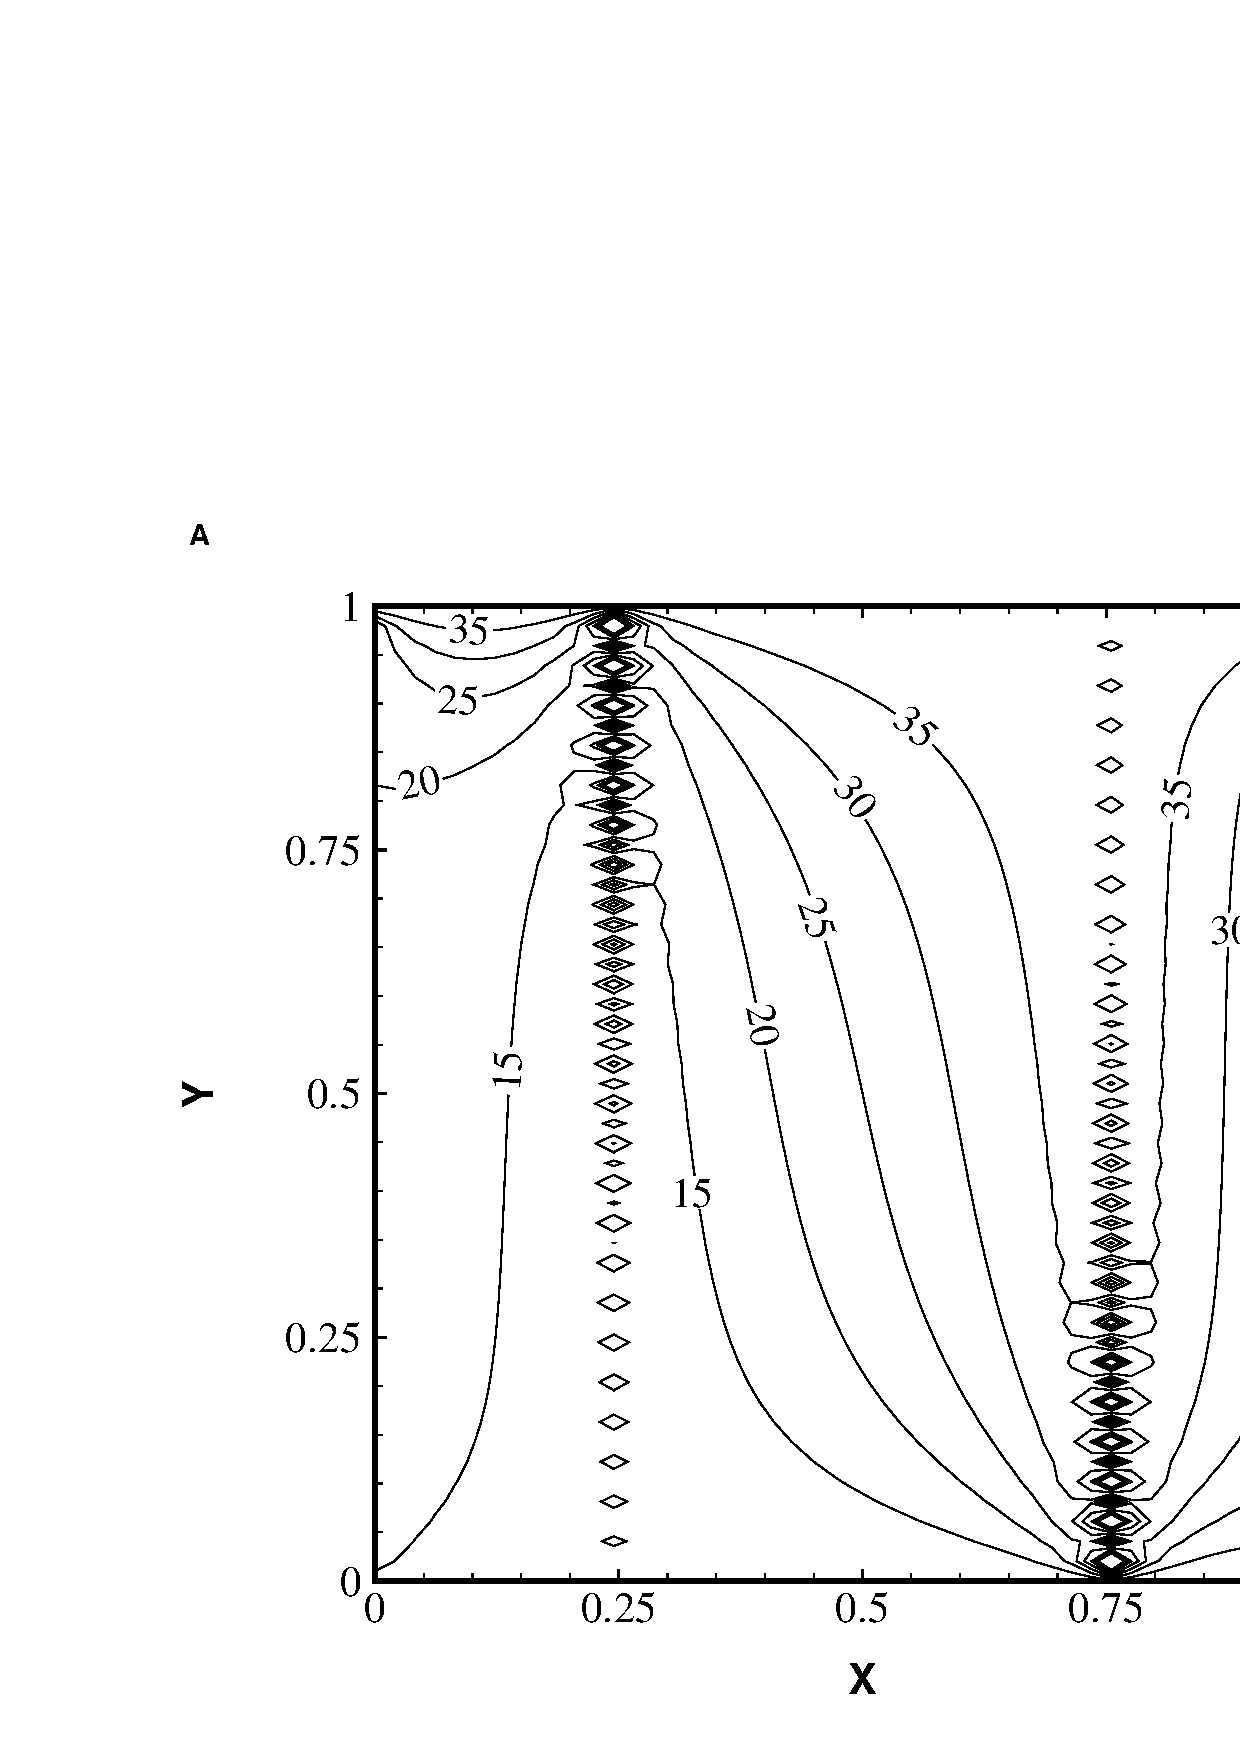
\includegraphics[width=0.9\columnwidth]{central.pdf}\\
   (a) Central\\[1.5em]
   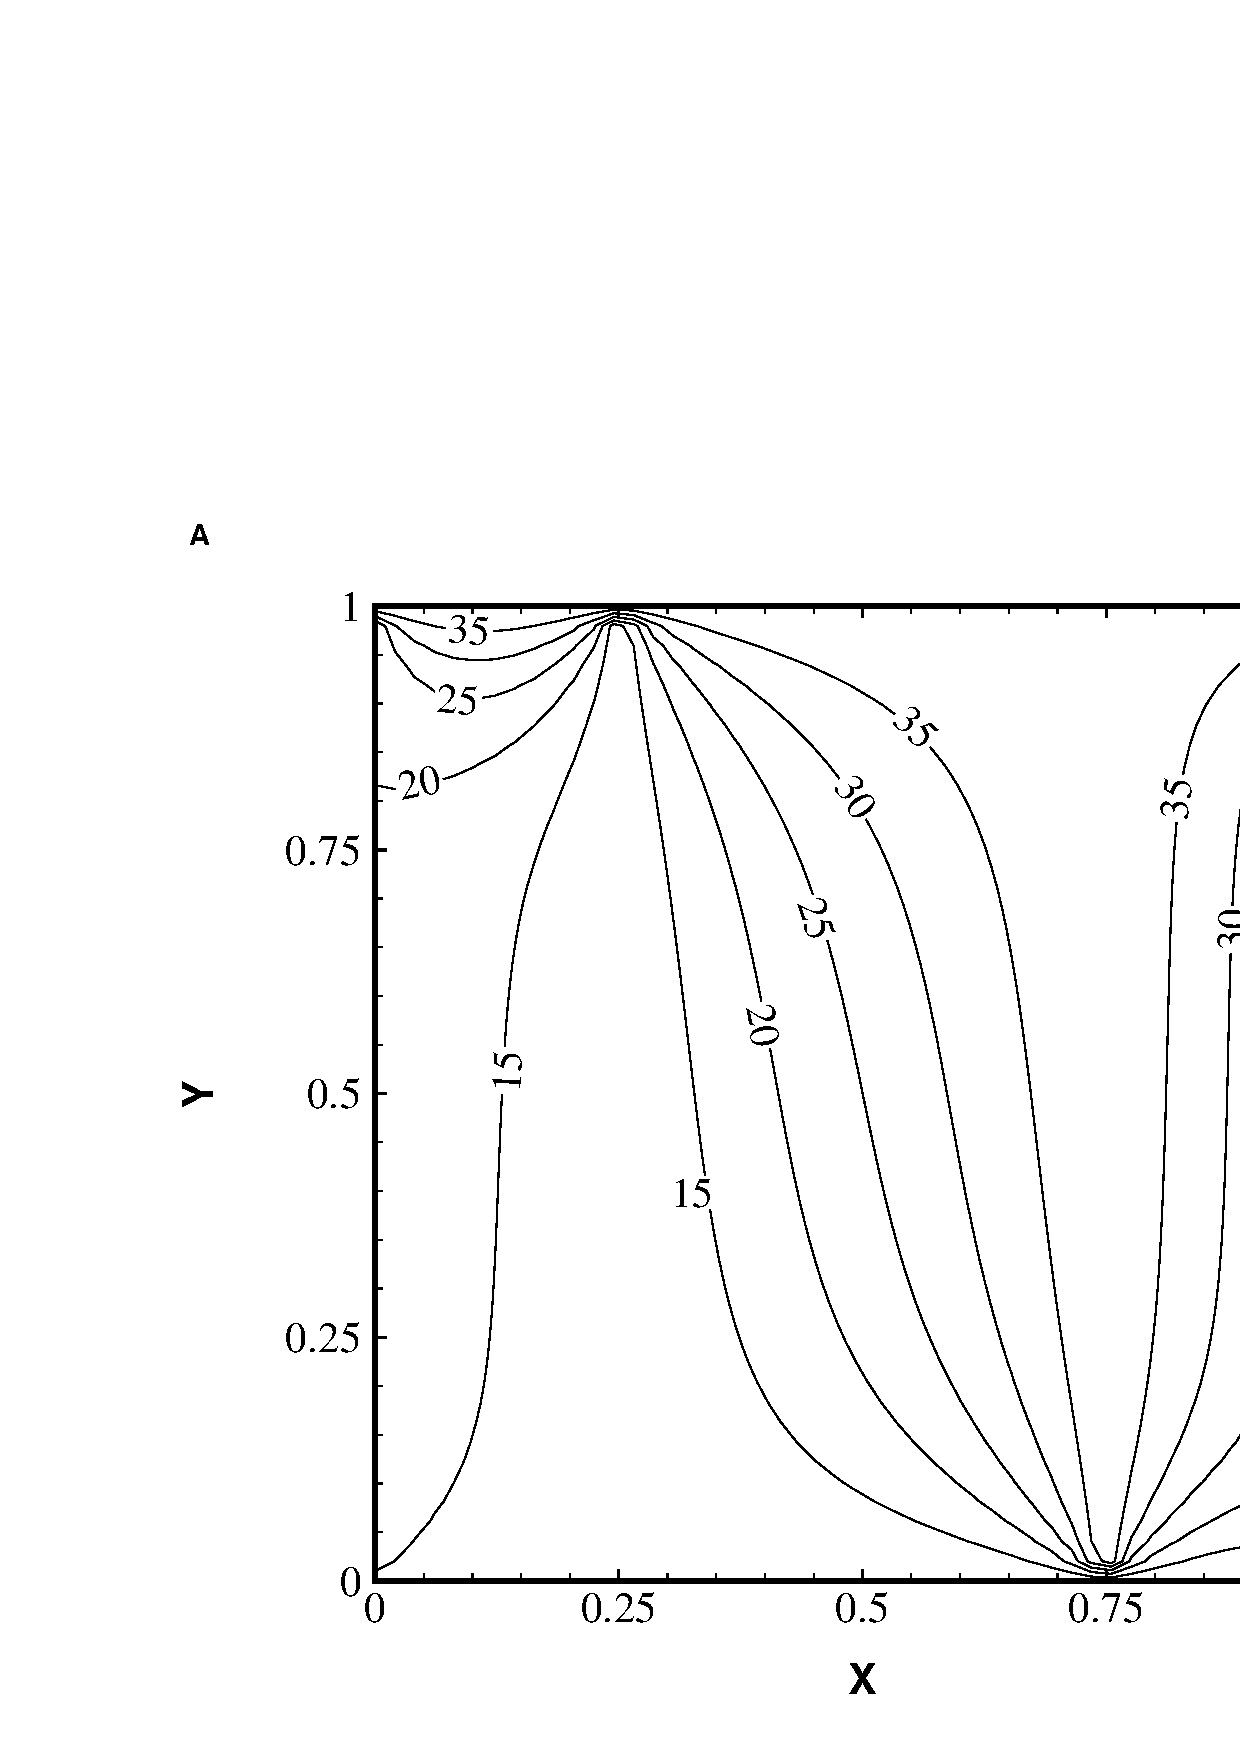
\includegraphics[width=0.9\columnwidth]{tvd.pdf}\\
   (b) TVD
   \end{center}
\figurecaption{Comparison of the potential contours (in volts) between the standard 9-point central-difference stencil and the proposed 13-point upwinded stencil.}
\label{fig:potentialcontours}
\end{figure}
%




The electric field potential equation can be obtained from the charged species mass and momentum conservation equations by assuming that the plasma is quasi-neutral and that the terms involving changes in inertia, viscous diffusion, pressure gradients, and collisions between charged particules are negligible compared to the terms involving electromagnetic forces and collisions between a charged particule and a neutral. Such can shown to be valid assumptions as long as the plasma remains weakly-ionized. Then, the potential equation becomes:
%
\begin{equation}
  \sum_i \frac{\partial}{\partial x_i} \sum_j  \wtilde{\sigma}_{ij} \left(\frac{\partial \phi}{\partial x_j}  - \left(\vec{v} \times \vec{B}\right)_j\right) =0
\end{equation}
%
where the  potential is defined such that $\vec{E}_j=-\partial \phi / \partial x_j$ and where the tensorial conductivity corresponds to:
%
\begin{equation}
\wtilde{\sigma}_{ij}=\sum_k |C_k| N_k \mu_k \left[Y_k\right]_{ij}
\end{equation}
%
with the matrix $Y_k$ equal to:
%
\begin{equation}
  Y_k = \left[\begin{array}{ccc} 
      1 & -s_k \mu_k \vec{B}_3  &  s_k \mu_k \vec{B}_2 \\
      s_k \mu_k \vec{B}_3 &  1 &  -s_k \mu_k \vec{B}_1 \\
      -s_k \mu_k \vec{B}_2 &  s_k \mu_k \vec{B}_1 & 1  \\
    \end{array} \right]^{-1}
\end{equation}
%
The existence of a potential for the electric field implies steady-state of the magnetic field. This is a reasonable assumption for weakly-ionized flowfields as long as the external magnetic field  does not vary in time. Indeed, the induced magnetic field can be considered negligible for weakly-ionized plasmas because the latter exhibit a low magnetic Reynolds number. For reasons that shall become apparent subsequently, the tensorial conductivity can also be written as a sum of a symmetric matrix and a skew-symmetric matrix:
%
\begin{equation}
  \wtilde{\sigma}=\wtilde{\sigma}^{\rm S} + \wtilde{\sigma}^{\rm SS}
\end{equation}
%
with the symmetric matrix equal to:
%
\begin{equation}
\wtilde{\sigma}^{\rm S}=\sum_k \frac{|C_k| N_k \mu_k}{1+\mu_k^2|\vec{B}|^2} 
\left[\begin{array}{ccc}
1+\mu_k^2\vec{B}_1^2
  & \mu_k^2 \vec{B}_1 \vec{B}_2 
  & \mu_k^2\vec{B}_1 \vec{B}_3  \alb
\mu_k^2 \vec{B}_1 \vec{B}_2  
  & 1+\mu_k^2\vec{B}_2^2
  & \mu_k^2\vec{B}_2 \vec{B}_3  \alb
\mu_k^2\vec{B}_1 \vec{B}_3  
  & \mu_k^2\vec{B}_2 \vec{B}_3 
  & 1+\mu_k^2\vec{B}_3^2
\end{array}
\right]
\end{equation}
%
and the skew-symmetric matrix equal to:	
%
\begin{equation}
\wtilde{\sigma}^{\rm SS}=\sum_k \frac{|C_k| N_k \mu_k}{1+\mu_k^2|\vec{B}|^2} 
\left[\begin{array}{ccc}
0 
 & s_k \mu_k  \vec{B}_3
 & -s_k \mu_k   \vec{B}_2 \alb
-s_k \mu_k  \vec{B}_3
 & 0
 &  s_k \mu_k \vec{B}_1 \alb
s_k \mu_k \vec{B}_2 
 & -s_k \mu_k \vec{B}_1
 & 0
\end{array}
\right]
\end{equation}
%
Then, after substituting the latter in the electric field potential equation, the following is obtained:
%
\begin{equation}
  \sum_i \frac{\partial}{\partial x_i} \sum_j   \left((\wtilde{\sigma}_{ij}^{\rm S}+\wtilde{\sigma}_{ij}^{\rm SS})\frac{\partial \phi}{\partial x_j}  - \wtilde{\sigma}_{ij}\left(\vec{v} \times \vec{B}\right)_j\right) =0
\end{equation}
%
It can be easily shown that the term function of the skew-symmetric conductivity tensor can be rewritten to:
%
\begin{equation}
\begin{array}{l}
\mfd\sum_i \frac{\partial}{\partial x_i} \sum_j \wtilde{\sigma}_{ij}^{\rm SS} \frac{\partial \phi}{\partial x_j} = 
 \sum_i \sum_j     \frac{\partial }{\partial x_j}\left(\frac{\partial \wtilde{\sigma}_{ij}^{\rm SS}}{\partial x_i} \phi\right) \alb\mfd
~~~~
- \phi \sum_i \sum_j \frac{\partial^2 \wtilde{\sigma}_{ij}^{\rm SS}}{\partial x_i \partial x_j}    
+\sum_i \sum_j \wtilde{\sigma}_{ij}^{\rm SS}     \frac{\partial^2 \phi}{\partial x_j \partial x_i} 
\end{array}
\end{equation}
%
The last two terms on the RHS will always be zero due to the commutativity of differentiation and due to the matrix $\wtilde{\sigma}^{\rm SS}$ being skew-symmetric and having diagonal elements equal to zero. Then, the electric field potential equation collapses to:
%
\begin{equation}
\sum_i \frac{\partial}{\partial x_i}   \sum_j   \left(\wtilde{\sigma}_{ij}^{\rm S}\frac{\partial \phi}{\partial x_j}  - \wtilde{\sigma}_{ij}\left(\vec{v} \times \vec{B}\right)_j\right) 
+ \sum_i \sum_j     \frac{\partial }{\partial x_j}\left(\frac{\partial \wtilde{\sigma}_{ij}^{\rm SS}}{\partial x_i} \phi\right) 
=0
\end{equation}
%
By substituting the $i$ and $j$ indices of the last term on the LHS and defining the wave speed associated with the skew-symmetric terms as
%
\begin{equation}
  a_i^{\rm SS} \equiv -\sum_j \frac{\partial \wtilde{\sigma}_{ji}^{\rm SS}}{\partial x_j}
\end{equation}
%
%
\begin{figure*}[t]
   \fontsizefigure
   \begin{center}
   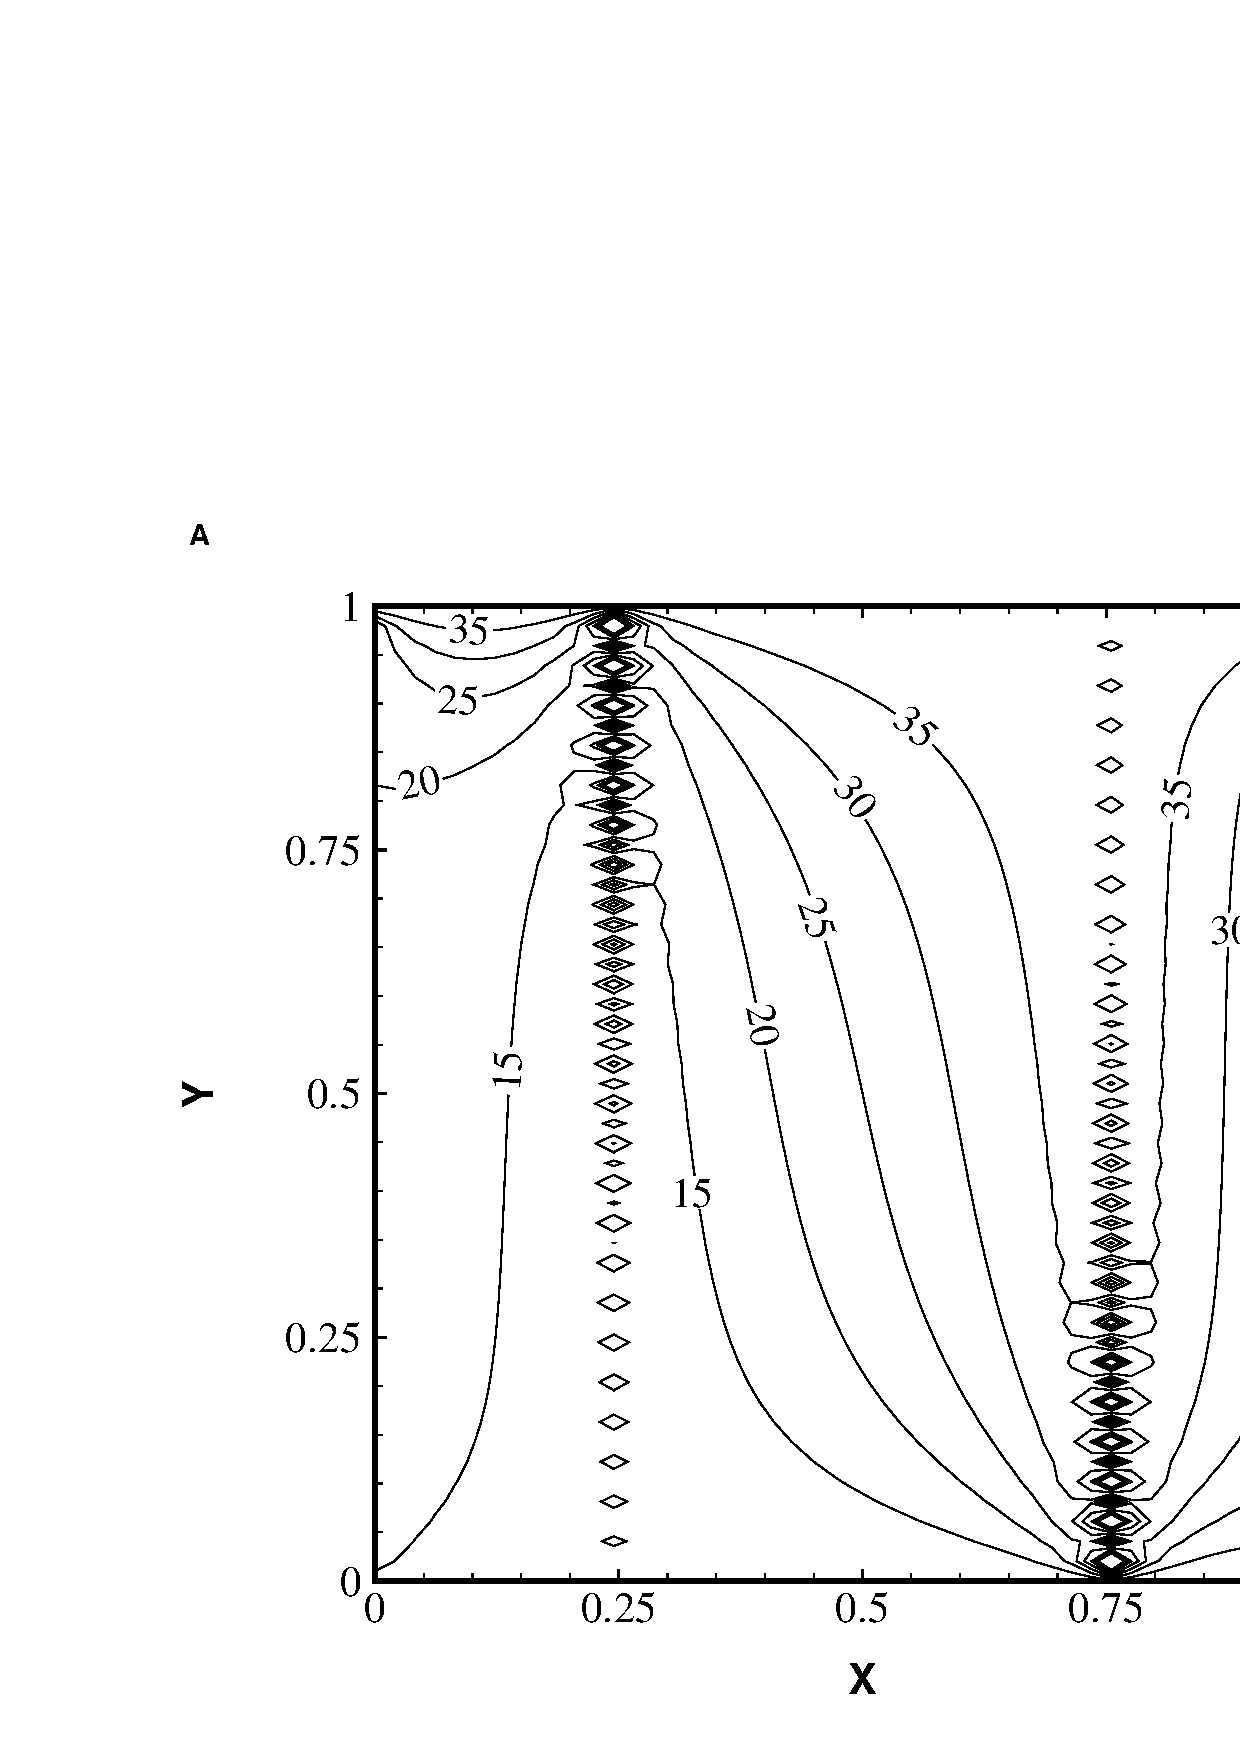
\includegraphics[width=0.9\columnwidth]{central.pdf}
   ~~~~
   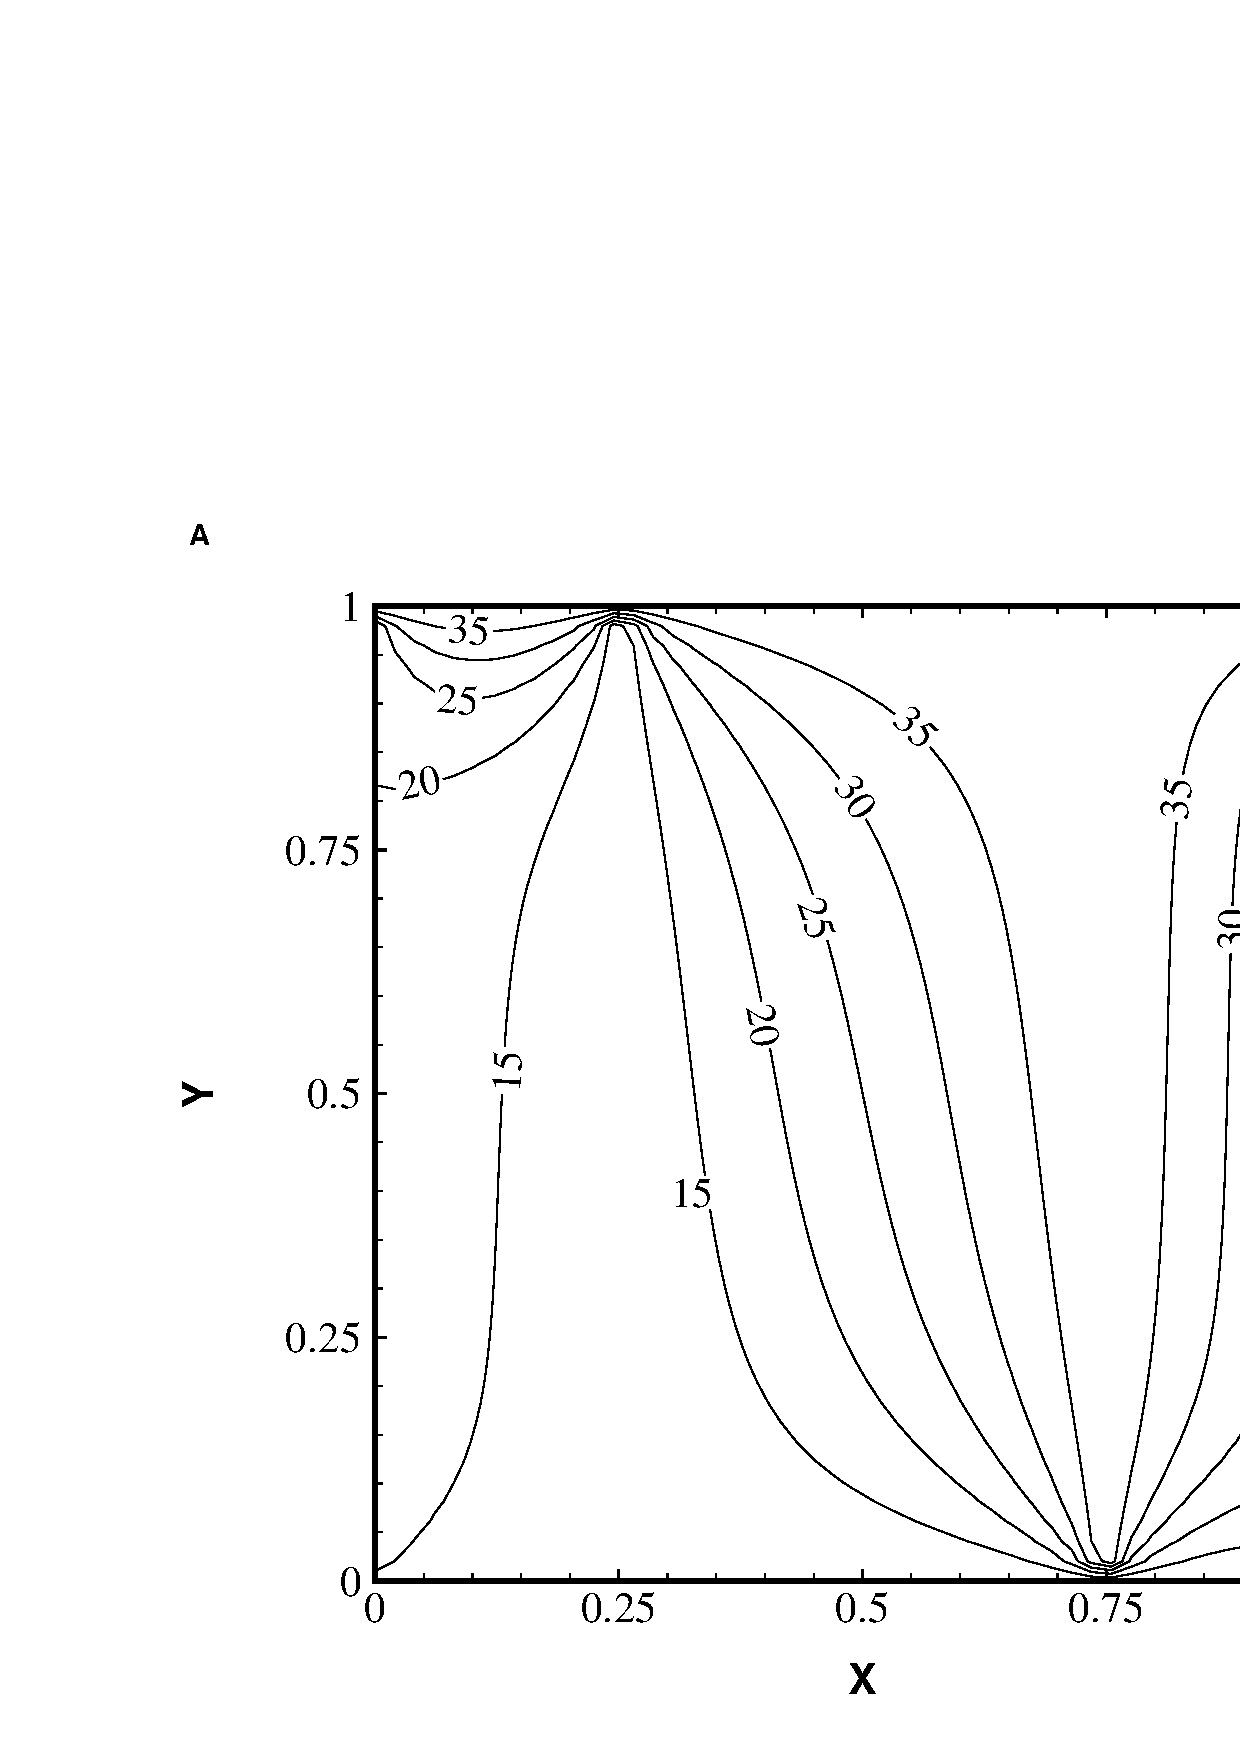
\includegraphics[width=0.9\columnwidth]{tvd.pdf}
   \end{center}
\figurecaption{Comparison of the potential contours (in volts) between the standard 9-point central-difference stencil and the proposed 13-point upwinded stencil.}
\label{fig:potentialcontours2}
\end{figure*}
%
the potential equation becomes:
%
\begin{equation}
\sum_i \frac{\partial}{\partial x_i}   \sum_j   \left(\wtilde{\sigma}_{ij}^{\rm S}\frac{\partial \phi}{\partial x_j}  - \wtilde{\sigma}_{ij}\left(\vec{v} \times \vec{B}\right)_j\right) 
- \sum_i     \frac{\partial }{\partial x_i}\left(a_i^{\rm SS} \phi\right) 
=0
\end{equation}
%
Interestingly, the skew-symmetric diffusion terms can be seen to collapse to a convection-like derivative, with the wave speed being proportional to the gradient of the conductivity. 


\section{Discretization of the Potential Equation ($\phi$)}

The electric field potential equation can  be expressed in discrete form as:
%
\begin{equation}
\sum_i \delta_{x_i}   \sum_j   \left(\wtilde{\sigma}_{ij}^{\rm S} \delta_{x_j} \phi  - \wtilde{\sigma}_{ij}\left(\vec{v} \times \vec{B}\right)_j\right) 
- \sum_i     \delta_{x_i}\left(a_i^{\rm SS} \phi\right) 
=0
\end{equation}
%
Because central differences cannot be used to discretize a convection derivative without introducing even-odd discoupling of the properties, it is necessary to use an upwinded stencil to discretize the
last derivative to prevent spurrious oscillations from forming.   
Therefore, in conservative form on a uniformly-spaced mesh, the discretization stencil of the skew-symmetric terms is set to:
%
%
\begin{equation}
\left[\delta_{x_i}\left( a_i^{\rm SS} \phi \right)\right]^{X_i} = \frac{\left( a_i^{\rm SS} \phi \right)^{X_i+\frac{1}{2}}-\left( a_i^{\rm SS} \phi \right)^{X_i-\frac{1}{2}}} {\Delta x_i}
\end{equation}
%
with the flux at the interface discretized using an upwinded stencil combined with a symmetric minmod TVD limiter \cite{jcp:1990:yee}:
%
\begin{equation}
\begin{array}{l}
\mfd
\left( a_i^{\rm SS} \phi \right)^{X_i+\frac{1}{2}}
=
\frac{1}{2}
\left(a_i^{\rm SS} \phi\right)^{X_i}
+
\frac{1}{2}
\left(a_i^{\rm SS} \phi\right)^{X_i+1}
\alb\mfd~~~~~~-\frac{1}{2}\left|a_i^{\rm SS}\right|^{X_i+\frac{1}{2}}\Delta\phi^{X_i+\frac{1}{2}}
\alb\mfd~~~~~~+\frac{1}{2}{\left|a_i^{\rm SS}\right|}^{X_i+\frac{1}{2}}~~{\rm minmod}\left(\Delta\phi^{X_i-\frac{1}{2}},~\Delta\phi^{X_i+\frac{1}{2}},~\Delta\phi^{X_i+\frac{3}{2}}
  \right)
\end{array}
\end{equation}
%
with $\Delta\phi^{X_i+\frac{1}{2}}\equiv\phi^{X_i+1}-\phi^{X_i}$ and where the minmod function returns the minimum of its arguments if the arguments are all positive, the maximum if the arguments are all negative, and zero if the arguments are of mixed signs. Such a stencil is monotonicity-preserving while being second-order accurate in regions where the properties vary smoothly. 
The other diffusion terms can be discretized with centered stencils as they do not pose any problem:
%
\begin{equation}
\left[ \delta_{x_i}    \left(\wtilde{\sigma}_{ij}^{\rm S} \delta_{x_j} \phi\right)\right]^{X_i}
=\frac{\left(\wtilde{\sigma}_{ij}^{\rm S} \delta_{x_j} \phi \right)^{X_i+\frac{1}{2}}-\left( \wtilde{\sigma}_{ij}^{\rm S} \delta_{x_j} \phi \right)^{X_i-\frac{1}{2}}} {\Delta x_i}
\end{equation}
%
where the flux at the interface would correspond to, when $i=j$:
%
\begin{equation}
\left(\wtilde{\sigma}_{ij}^{\rm S} \delta_{x_j} \phi \right)^{X_i+\frac{1}{2}}
=
\left(\wtilde{\sigma}_{ii}^{\rm S}\right)^{X_i+\frac{1}{2}}
\frac{
\phi^{X_i+1}-\phi^{X_i}
}{
\Delta x_i
}
\end{equation}
%
and to, when $i\ne j$:
%
\begin{equation}
\begin{array}{l}
\mfd\left(\wtilde{\sigma}_{ij}^{\rm S} \delta_{x_j} \phi \right)^{X_i+\frac{1}{2}}
=
\left(\wtilde{\sigma}_{ij}^{\rm S}\right)^{X_i+\frac{1}{2},X_j}
\alb\mfd
~~~~~\times\frac{
\phi^{X_i,X_j+1}+\phi^{X_i+1,X_j+1}-\phi^{X_i,X_j-1}-\phi^{X_i+1,X_j-1}
}{
4 \Delta x_j
}
\end{array}
\end{equation}
%


\section{Test Cases}

While the numerical method outlined above is written in general form and is applicable to plasmas in which both electrons and ions can carry current, the test case here presented is limited for simplicity to a plasma in which the current is carried solely by the electrons. Then, the symmetric conductivity matrix simplifies to:
%
\begin{equation}
  \wtilde{\sigma}^{\rm S}\rightarrow \frac{\sigma}{1+\beta_{\rm e}^2}\left[ 
\begin{array}{ccc}
 1+\beta_{\rm e}^2 \bar{\vec{B}}_1^2 
 &  \beta_{\rm e}^2\bar{\vec{B}}_1 \bar{\vec{B}}_2
 &  \beta_{\rm e}^2\bar{\vec{B}}_1 \bar{\vec{B}}_3 \alb
 \beta_{\rm e}^2\bar{\vec{B}}_1 \bar{\vec{B}}_2
 &  1+\beta_{\rm e}^2\bar{\vec{B}}_2^2 
 &  \beta_{\rm e}^2\bar{\vec{B}}_2 \bar{\vec{B}}_3 \alb
 \beta_{\rm e}^2\bar{\vec{B}}_1 \bar{\vec{B}}_3
 &  \beta_{\rm e}^2\bar{\vec{B}}_2 \bar{\vec{B}}_3
 &  1+\beta_{\rm e}^2\bar{\vec{B}}_3^2 
\end{array}
\right]
\end{equation}
%
and the skew-symmetric matrix becomes:
%
\begin{equation}
  \wtilde{\sigma}^{\rm SS}\rightarrow \frac{ \sigma }{1+\beta_{\rm e}^2}\left[ 
\begin{array}{ccc}
0
 & -\beta_{\rm e}\bar{\vec{B}}_3
 & \beta_{\rm e}\bar{\vec{B}}_2 \alb
   \beta_{\rm e}\bar{\vec{B}}_3
 & 0
 & -\beta_{\rm e}\bar{\vec{B}}_1 \alb
-\beta_{\rm e}\bar{\vec{B}}_2
 & \beta_{\rm e}\bar{\vec{B}}_1
 & 0
\end{array}
\right]
\end{equation}
%
From the latter, it is apparent that the skew symmetric terms are negligible when the Hall parameter is much less than unity. Additionally, as was  shown in the previous section, the skew symmetric terms collapse to zero when there is no gradient of the conductivity. 
Therefore, in order to test adequately the proposed discretization scheme,  the Hall parameter and the conductivity gradient are here set sufficiently high that the skew-symmetric terms  predominate over the symmetric terms. 

The  test case consists of a two-dimensional domain with Dirichlet boundary conditions:
%
\begin{equation}
 \phi_{x=0}=20~{\rm V},~~\phi_{x=1\,{\rm m}}=20~{\rm V}
,~~\phi_{y=0}=10~{\rm V},~~\phi_{y=1\,{\rm m}}=40~{\rm V}
\end{equation}
% 
with the Hall parameter  fixed to 20, the bulk gas velocity to zero, and the conductivity such that it exhibits a strong gradient in some regions of the domain: 
%
\begin{equation}
\sigma=
\left\{
\begin{array}{ll}
 1.0~{\rm S/m}&{\rm for~}0.25~{\rm m} \le x \le 0.75~{\rm m}\alb
 0.0001~{\rm S/m}&{\rm otherwise}
\end{array}
\right.
\end{equation}
% 
Even thus the gradient of the conductivity is high and  the Hall parameter is high, spurious oscillations may still not occur. Indeed, the skew-symmetric terms may  become  negligible for certain orientations of the magnetic field vector. It can be easily shown that this would occur when the magnetic field vector lies within the plane made by the potential gradient vector and the conductivity gradient vector. For this reason and because it is desired to test the monotonicity-preserving capability of the proposed scheme under the most stringent conditions, the normalized magnetic field vector is here fixed perpendicular to the computational domain:
%
\begin{equation}
\bar{B}=(0,~0,~1)
\end{equation}
%
The mesh is made of 50 grid lines along each dimension and the solution is advanced iteratively using an implicit approximate factorization algorithm until convergence is attained. The solution is considered converged when the discrete residual on all nodes falls below a given threshold typically set to $10^{-3}$. This is verified to be sufficiently small to yield potential contours that are visually indistinguishable from those obtained using a residual convergence threshold set to machine tolerance (about $10^{-13}$).


A comparison between the potential contours obtained with the standard 9-point central-difference stencil and the proposed 13-point upwinded stencil is shown in Fig.\ \ref{fig:potentialcontours}. As expected, the use of the standard central-difference stencil is seen to introduce severe spurrious oscillations of the electric field potential in the regions where the gradient of the conductivity is high. Such aphysical oscillations of the potential are completely removed when the upwinded stencil is used.
 While not shown here for brevity, several other test cases confirm the monotonicity-preserving capability and second-order accuracy of the proposed method.   


\section{Conclusions}

There are two significant results of the research described in this paper. First, only a small range of values for the cross-diffusion coefficient $\sigma_d$ exists that yields satisfactory spreading rates for free shear flows. 
The discretization of the electric field potential equation is here demonstrated to require the use of upwinded stencils in order to yield a solution free of spurrious oscillations. The use of upwinded stencils is seen to be necessary when the skew-symmetric terms part of the tensor conductivity matrix predominate over the other terms. This is shown to be the case when three conditions are met: (i) the Hall parameter is high, (ii) the conductivity exhibits a significant spatial gradient, and (iii) the magnetic field vector has a component perpendicular to both the potential gradient vector and the conductivity gradient vector. 

A new discretization stencil for the potential equation is here proposed, spanning 13 grid points in 2D and 33 grid point in 3D. The stencil consists of a minmod TVD upwinded scheme for the skew-symmetric terms and a central difference stencil for the other terms. The proposed method is monotonicity-preserving  and, in regions where the properties vary smoothly, reaches second-order accuracy. Several test cases were performed to evaluate the performance of the proposed method compared to the standard central-difference scheme. In all cases, including those with the most stringent conditions, the use of the proposed method results in a complete removal of the aphysical oscillations.  

\appendix
\section{Appendix Test}   

The proposed upwinded stencil  is recommended for all flow problems in which the electric field potential equation is solved in coupled form with the Navier Stokes equations, irrespectively of the value of the average Hall parameter. Indeed, even if the Hall parameter remains low on average, it can attain values well exceeding unity in some flow regions due to Joule heating or some other phenomenon decreasing locally the gas density (on which the Hall parameter inversely depends).  
%
\begin{equation}
a=b+c
\end{equation}
%

\bibliography{all}
\bibliographystyle{aiaa}

    \end{document}
